% 05_lerobot.tex - Physical Robot Module
% AlohaMini Codebase Documentation

\section{LeRobot Module (Physical Robot)}

% ============================================
% SLIDE: Module Overview
% ============================================
\begin{frame}{software/ Module Overview}
\begin{columns}
\begin{column}{0.4\textwidth}
    \textbf{Purpose:} Physical robot control via LeRobot framework

    \vspace{0.2cm}

    \textbf{Key Files:}
    \begin{itemize}
        \item \filepath{lekiwi.py} (642 lines)
        \item \filepath{config\_lekiwi.py} (114 lines)
        \item \filepath{lift\_axis.py} (217 lines)
    \end{itemize}

    \vspace{0.2cm}

    \textbf{Dependencies:}
    \begin{itemize}
        \item LeRobot framework
        \item Feetech motors (STS3215)
        \item OpenCV cameras
    \end{itemize}
\end{column}
\begin{column}{0.6\textwidth}
    \centering
    \begin{tikzpicture}[scale=0.8, transform shape]
        % Main robot class
        \node[class, text width=4cm, minimum height=1.2cm] (lekiwi) at (0,0) {
            \textbf{LeKiwi}\\
            \footnotesize extends Robot
        };

        % Components
        \node[submodule, text width=2cm, below left=1cm and 0.3cm of lekiwi] (left) {
            Left Bus
        };
        \node[submodule, text width=2cm, below=1cm of lekiwi] (right) {
            Right Bus
        };
        \node[submodule, text width=2cm, below right=1cm and 0.3cm of lekiwi] (lift) {
            LiftAxis
        };

        % Config
        \node[class, text width=2.5cm, above=0.8cm of lekiwi] (config) {
            LeKiwiConfig
        };

        % Arrows
        \draw[arrow] (config) -- (lekiwi);
        \draw[arrow] (lekiwi) -- (left);
        \draw[arrow] (lekiwi) -- (right);
        \draw[arrow] (lekiwi) -- (lift);
    \end{tikzpicture}
\end{column}
\end{columns}
\end{frame}

% ============================================
% SLIDE: Hardware Architecture
% ============================================
\begin{frame}{AlohaMini Hardware Architecture}
\centering
\begin{tikzpicture}[scale=0.8, transform shape]
    % Robot outline
    \draw[rounded corners=8pt, thick, fill=gray!10] (-3.5,-1.2) rectangle (3.5,3.5);
    \node[above, font=\bfseries\small] at (0,3.5) {AlohaMini Physical Robot};

    % Mobile base
    \draw[fill=gray!30, rounded corners=3pt] (-2.5,-0.8) rectangle (2.5,0);
    \node[font=\footnotesize] at (0,-0.4) {Omniwheel Base (3)};

    % Wheels
    \draw[fill=black!60] (-1.8,-1) circle (0.18);
    \draw[fill=black!60] (1.8,-1) circle (0.18);
    \draw[fill=black!60] (0,-1) circle (0.18);

    % Lift column
    \draw[fill=blue!20] (-0.2,0) rectangle (0.2,2);
    \node[rotate=90, font=\tiny] at (0,1) {Lift};

    % Arm platform
    \draw[fill=gray!20] (-2,2) rectangle (2,2.4);

    % Left arm
    \draw[link] (-1.2,2.4) -- (-2,3);
    \node[joint, minimum size=0.25cm] at (-1.2,2.4) {};
    \node[joint, minimum size=0.25cm] at (-2,3) {};
    \node[font=\tiny] at (-2,3.3) {Left (6)};

    % Right arm
    \draw[link] (1.2,2.4) -- (2,3);
    \node[joint, minimum size=0.25cm] at (1.2,2.4) {};
    \node[joint, minimum size=0.25cm] at (2,3) {};
    \node[font=\tiny] at (2,3.3) {Right (6)};

    % Bus connections (right side)
    \node[draw, rounded corners, fill=yellow!20, text width=1.8cm, font=\tiny, align=center] (leftbus) at (5.5,2) {
        \textbf{Left Bus}\\
        Arm (6)\\
        Base (3)\\
        Lift (1)
    };
    \node[draw, rounded corners, fill=orange!20, text width=1.8cm, font=\tiny, align=center, below=0.2cm of leftbus] (rightbus) {
        \textbf{Right Bus}\\
        Arm (6)
    };

    % Connection lines
    \draw[dashed, gray, thin] (2,3) -- (rightbus.west);
    \draw[dashed, gray, thin] (-2,3) -- (leftbus.west);
\end{tikzpicture}
\end{frame}

% ============================================
% SLIDE: Motor Configuration
% ============================================
\begin{frame}[fragile]{LeKiwi - Motor Configuration}
\begin{lstlisting}[basicstyle=\ttfamily\scriptsize]
self.left_bus = FeetechMotorsBus(
    port=self.config.left_port,
    motors={
        # Left arm joints (6 DOF)
        "arm_left_shoulder_pan": Motor(1, "sts3215", norm_mode),
        "arm_left_shoulder_lift": Motor(2, "sts3215", norm_mode),
        "arm_left_elbow_flex": Motor(3, "sts3215", norm_mode),
        "arm_left_wrist_flex": Motor(4, "sts3215", norm_mode),
        "arm_left_wrist_roll": Motor(5, "sts3215", norm_mode),
        "arm_left_gripper": Motor(6, "sts3215", RANGE_0_100),
        # Mobile base (3 wheels)
        "base_left_wheel": Motor(8, "sts3215", RANGE_M100_100),
        "base_back_wheel": Motor(9, "sts3215", RANGE_M100_100),
        "base_right_wheel": Motor(10, "sts3215", RANGE_M100_100),
        # Lift mechanism
        "lift_axis": Motor(11, "sts3215", DEGREES),
    },
)
\end{lstlisting}
\end{frame}

% ============================================
% SLIDE: State Features
% ============================================
\begin{frame}{LeKiwi - State/Action Features}
\begin{columns}
\begin{column}{0.5\textwidth}
    \textbf{State Features (16 DOF):}
    \begin{itemize}
        \item \code{arm\_left\_*.pos} (6)
        \item \code{arm\_right\_*.pos} (6)
        \item \code{x.vel, y.vel, theta.vel} (3)
        \item \code{lift\_axis.height\_mm} (1)
    \end{itemize}

    \vspace{0.3cm}

    \textbf{Camera Features (5):}
    \begin{itemize}
        \item head\_top, head\_back, head\_front
        \item wrist\_left, wrist\_right
        \item Resolution: 640$\times$480
    \end{itemize}
\end{column}
\begin{column}{0.5\textwidth}
    \begin{table}
    \centering
    \footnotesize
    \begin{tabular}{lr}
    \toprule
    \textbf{Component} & \textbf{DOF} \\
    \midrule
    Left Arm & 6 \\
    Right Arm & 6 \\
    Base Velocity & 3 \\
    Lift Height & 1 \\
    \midrule
    \textbf{Total} & \textbf{16} \\
    \bottomrule
    \end{tabular}
    \end{table}

    \vspace{0.3cm}

    \begin{block}{Action = State}
    Action features mirror state features for teleoperation recording.
    \end{block}
\end{column}
\end{columns}
\end{frame}

% ============================================
% SLIDE: Omniwheel Kinematics
% ============================================
\begin{frame}{Omniwheel Base Kinematics}
\begin{columns}
\begin{column}{0.45\textwidth}
    \centering
    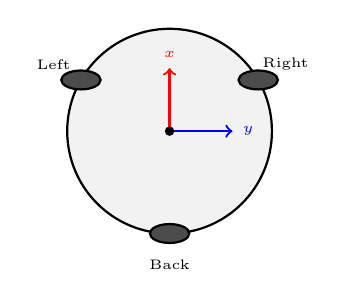
\begin{tikzpicture}[scale=1.0, transform shape]
        % Robot base circle
        \draw[thick, fill=gray!10] (0,0) circle (1.3);

        % Wheel positions
        \foreach \angle in {150, 270, 30} {
            \draw[fill=black!70, thick] (\angle:1.3) ellipse (0.25 and 0.12);
        }

        % Wheel labels
        \node[font=\tiny] at (150:1.7) {Left};
        \node[font=\tiny] at (270:1.7) {Back};
        \node[font=\tiny] at (30:1.7) {Right};

        % Coordinate frame
        \draw[->, thick, red] (0,0) -- (0,0.8) node[above, font=\tiny] {$x$};
        \draw[->, thick, blue] (0,0) -- (0.8,0) node[right, font=\tiny] {$y$};

        % Center
        \fill (0,0) circle (0.06);
    \end{tikzpicture}
\end{column}
\begin{column}{0.55\textwidth}
    \textbf{Inverse Kinematics:}

    Wheel angles: $\phi_i = [150°, 270°, 30°]$

    \vspace{0.2cm}

    Kinematic matrix:
    \[M = \begin{bmatrix}
        \cos\phi_1 & \sin\phi_1 & R \\
        \cos\phi_2 & \sin\phi_2 & R \\
        \cos\phi_3 & \sin\phi_3 & R
    \end{bmatrix}\]

    Body to wheel: $\vec{\omega} = \frac{M \cdot \vec{v}}{r}$

    \vspace{0.2cm}

    \textbf{Parameters:}
    \begin{itemize}
        \item $r_{wheel} = 0.05m$
        \item $R_{base} = 0.125m$
    \end{itemize}
\end{column}
\end{columns}
\end{frame}

% ============================================
% SLIDE: Body to Wheel Conversion
% ============================================
\begin{frame}[fragile]{Body to Wheel Conversion}
\begin{lstlisting}[basicstyle=\ttfamily\scriptsize]
def _body_to_wheel_raw(self, x, y, theta, wheel_radius=0.05,
                       base_radius=0.125, max_raw=3000):
    """Convert body velocities (x, y, theta) to wheel raw commands."""
    theta_rad = theta * (np.pi / 180.0)
    velocity_vector = np.array([-x, -y, theta_rad])

    # Wheel mounting angles with -90 deg offset
    angles = np.radians(np.array([240, 0, 120]) - 90)
    m = np.array([[np.cos(a), np.sin(a), base_radius] for a in angles])

    # Compute wheel speeds
    wheel_linear_speeds = m.dot(velocity_vector)
    wheel_angular_speeds = wheel_linear_speeds / wheel_radius
    wheel_degps = wheel_angular_speeds * (180.0 / np.pi)

    # Scale if exceeds max_raw ...
    wheel_raw = [self._degps_to_raw(deg) for deg in wheel_degps]
    return {"base_left_wheel": wheel_raw[0], ...}
\end{lstlisting}
\end{frame}

% ============================================
% SLIDE: LiftAxis Config
% ============================================
\begin{frame}[fragile]{LiftAxis - Configuration}
\begin{columns}
\begin{column}{0.55\textwidth}
\begin{lstlisting}[basicstyle=\ttfamily\scriptsize]
@dataclass
class LiftAxisConfig:
    enabled: bool = True
    name: str = "lift_axis"
    motor_id: int = 11

    # Lead screw parameters
    lead_mm_per_rev: float = 84
    soft_min_mm: float = 0.0
    soft_max_mm: float = 600

    # Homing parameters
    home_down_speed: int = 1300
    home_stall_current_ma: int = 150

    # Velocity control
    kp_vel: float = 300
    v_max: int = 1300
    dir_sign: int = -1
\end{lstlisting}
\end{column}
\begin{column}{0.45\textwidth}
    \textbf{Key Features:}
    \begin{itemize}
        \item Multi-turn tracking
        \item Velocity closed-loop
        \item Automatic homing
        \item Soft limits
    \end{itemize}

    \vspace{0.3cm}

    \textbf{Position Calc:}
    \begin{align*}
        h_{mm} &= (\theta - \theta_0) \\
               &\quad \times \frac{lead}{360°}
    \end{align*}
\end{column}
\end{columns}
\end{frame}

% ============================================
% SLIDE: LiftAxis Homing
% ============================================
\begin{frame}{LiftAxis - Homing Procedure}
\begin{columns}
\begin{column}{0.5\textwidth}
    \textbf{Homing Algorithm:}
    \begin{enumerate}
        \item Drive down at \code{home\_down\_speed}
        \item Monitor current (6.5x scale)
        \item Detect stall (\textgreater 1500mA)
        \item Set current position as z=0
    \end{enumerate}
\end{column}
\begin{column}{0.5\textwidth}
    \textbf{Parameters:}
    \begin{itemize}
        \item Timeout: 30 seconds
        \item Poll rate: 50ms
        \item Stall threshold: 2 consecutive
        \item Current limit: 1500 mA
    \end{itemize}
\end{column}
\end{columns}
\end{frame}

% ============================================
% SLIDE: Observation Flow
% ============================================
\begin{frame}{LeKiwi - Observation \& Action Flow}
\centering
\begin{tikzpicture}[scale=0.9, transform shape, node distance=1.2cm]
    % Observation flow
    \node[module, text width=2.5cm] (motors) at (0,0) {Motors\\(sync\_read)};
    \node[module, text width=2.5cm, right=1.5cm of motors] (cameras) {Cameras\\(async\_read)};
    \node[module, text width=3.5cm, below=1.2cm of $(motors)!0.5!(cameras)$] (obs) {Observation Dict};

    % Action flow
    \node[module, text width=3.5cm, below=of obs] (action) {Action Dict};
    \node[module, text width=2cm, below left=1.2cm and 0.3cm of action] (arm) {Arms\\(Position)};
    \node[module, text width=2cm, below=1.2cm of action] (base) {Base\\(Velocity)};
    \node[module, text width=2cm, below right=1.2cm and 0.3cm of action] (lift) {Lift\\(Height)};

    % Arrows
    \draw[flow] (motors) -- (obs);
    \draw[flow] (cameras) -- (obs);
    \draw[flow] (obs) -- node[right, font=\footnotesize] {Policy / Teleop} (action);
    \draw[flow] (action) -- (arm);
    \draw[flow] (action) -- (base);
    \draw[flow] (action) -- (lift);
\end{tikzpicture}
\end{frame}

% ============================================
% SLIDE: Safety Features
% ============================================
\begin{frame}{LeKiwi - Safety Features}
\begin{columns}
\begin{column}{0.5\textwidth}
    \textbf{1. Overcurrent Protection}
    \begin{itemize}
        \item Default limit: 2000 mA
        \item Scale factor: 6.5 (STS3215)
        \item Emergency stop on exceed
        \item Auto-disconnect
    \end{itemize}

    \vspace{0.3cm}

    \textbf{2. Position Safety}
    \begin{itemize}
        \item \code{max\_relative\_target}
        \item Caps relative motion magnitude
        \item Prevents sudden jumps
    \end{itemize}
\end{column}
\begin{column}{0.5\textwidth}
    \textbf{3. Lift Soft Limits}
    \begin{itemize}
        \item \code{soft\_min\_mm = 0}
        \item \code{soft\_max\_mm = 600}
        \item Velocity blocked at limits
    \end{itemize}

    \vspace{0.3cm}

    \textbf{4. Watchdog (Client Mode)}
    \begin{itemize}
        \item Timeout: 1500 ms
        \item Stops robot if no command
        \item Network disconnection safety
    \end{itemize}
\end{column}
\end{columns}
\end{frame}

% ============================================
% SLIDE: Calibration Process
% ============================================
\begin{frame}{Calibration Process}
\begin{columns}
\begin{column}{0.5\textwidth}
    \textbf{Dual-Bus Calibration:}
    \begin{enumerate}
        \item Disable torque on arm motors
        \item Move LEFT arm to middle
        \item Record half-turn homing offset
        \item Move through full ROM
        \item Record min/max positions
        \item Repeat for RIGHT arm
        \item Merge and save calibration
    \end{enumerate}
\end{column}
\begin{column}{0.5\textwidth}
    \centering
    \begin{tikzpicture}[scale=0.75, transform shape, node distance=0.7cm]
        \node[module, text width=2.5cm] (start) {Start};
        \node[module, text width=2.5cm, below=of start] (left) {Left Arm};
        \node[module, text width=2.5cm, below=of left] (right) {Right Arm};
        \node[module, text width=2.5cm, below=of right] (merge) {Merge};
        \node[module, text width=2.5cm, below=of merge] (save) {Save};

        \draw[flow] (start) -- (left);
        \draw[flow] (left) -- (right);
        \draw[flow] (right) -- (merge);
        \draw[flow] (merge) -- (save);

        \node[submodule, text width=1.8cm, right=0.3cm of left, font=\tiny] (base) {Base: 0-4095};
        \draw[dashed, gray] (left) -- (base);
    \end{tikzpicture}
\end{column}
\end{columns}
\end{frame}

% ============================================
% SLIDE: LeKiwiConfig
% ============================================
\begin{frame}[fragile]{LeKiwiConfig}
\begin{lstlisting}[basicstyle=\ttfamily\scriptsize]
@RobotConfig.register_subclass("lekiwi")
@dataclass
class LeKiwiConfig(RobotConfig):
    left_port: str = "/dev/am_arm_follower_left"
    right_port: str = "/dev/am_arm_follower_right"
    disable_torque_on_disconnect: bool = True
    max_relative_target: int | None = None
    cameras: dict[str, CameraConfig] = field(default_factory=...)
    use_degrees: bool = False
\end{lstlisting}

\vspace{0.3cm}

\textbf{Camera Device Paths:}
\begin{itemize}
    \item \code{/dev/am\_camera\_head\_top}
    \item \code{/dev/am\_camera\_head\_back}, \code{head\_front}
    \item \code{/dev/am\_camera\_wrist\_left}, \code{wrist\_right}
\end{itemize}
\end{frame}

% ============================================
% SLIDE: Module Summary
% ============================================
\begin{frame}{LeRobot Module Summary}
\begin{columns}
\begin{column}{0.5\textwidth}
    \textbf{Key Classes:}
    \begin{itemize}
        \item \code{LeKiwi} - Robot interface
        \item \code{LeKiwiConfig} - Configuration
        \item \code{LiftAxis} - Z-axis controller
    \end{itemize}

    \vspace{0.3cm}

    \textbf{Hardware:}
    \begin{itemize}
        \item Feetech STS3215 servos
        \item FeetechMotorsBus
        \item 5 OpenCV cameras
    \end{itemize}
\end{column}
\begin{column}{0.5\textwidth}
    \textbf{Control Modes:}
    \begin{table}
    \centering
    \footnotesize
    \begin{tabular}{ll}
    \toprule
    \textbf{Component} & \textbf{Mode} \\
    \midrule
    Arms & Position \\
    Base wheels & Velocity \\
    Lift axis & Velocity \\
    \bottomrule
    \end{tabular}
    \end{table}

    \vspace{0.3cm}

    \textbf{Control Loop:} 30-50 Hz
\end{column}
\end{columns}
\end{frame}

